\documentclass{article}
\usepackage{graphicx} % Required for inserting images
\usepackage{amsmath} 
\usepackage{float} % For precise figure placement with [H]


\title{MaxFlow Report -inf05016}
\author{Victor Scherer Putrich}
\date{March 2024}

\begin{document}

\maketitle


\section{Collected Information}

For this work, we are going to analyze several measures regarding the correctness of the Edmonds-Karp algorithm, considering upper bounds on the number of times each edge was a critical edge; and also regarding the number of iterations and operations in Breadth-First Search (BFS) for pushing flows. For keeping the scope practical we are going to use only Mesh graph, without exploring other topologies.

The measures mentioned in the assignment for Edmonds-Karp correctness were:
\begin{itemize}
    \item $C$: for comparing the number of critical arcs with the number of total edges. (Should be lower than 1)
    \item $r_a$: as a ratio for the number of times a single arc is critical compared to its upper bound $n/2$.
    \item $\bar{r}$: as an average on criticality, given by $r_a$ for all arcs with the total number of arcs. (Should be lower than 1)
\end{itemize}

For BFS we have:
\begin{itemize}
    \item $t_i$: ratio on the number of visited edges $m'$ on iteration $i$ divided by the total number of edges $m$. (Should be lower than 1) 
    \item $s_i$: ratio on the number of visited edges $n'$ on iteration $i$ divided by the total number of edges $n$. (Should be lower than 1) 
    \item $I$: as the number of iterations, having an upper bound of $\bar{r}/2nm$, which can be a lower value in case there are several critical edges in a single iteration.
\end{itemize}

We are going to include the use of the pessimistic complexity measure; and compare how increasing the number of rows and columns affects the number of augmentations, the number of BFS internal operations, and also the maximum flow.

\section{Experiment}

Our experiments were conducted on an AMD Ryzen 5 3600 6-Core Processor@3.6 GHZ, DDR4 RAM, and Operational System Ubuntu 22.04LTS.

We pick a Mesh graph which uses the number of rows and columns as parameters to define the number of vertices and edges. We ran each parameter with values using the following sequence [2 4 8 16 32 64 128] with maximum flow capacities of [100,1000,10000,100000] and tested every possible configuration row x columns. For each graph, we set the X-axis as a row, or column, and compare it over several measurements. In case the graph uses a row on the x-axis, we plot each column value into the graph, and for each graph using columns, we plot each row value into the graph.

As an example, we have Figure~\ref{fig:edges-example}, where we show the number of edges compared to the number of rows (left image), and columns (right image). For each graph type, we plot the secondary argument, \emph{\#Columns} and \emph{\#Rows}. This first figure indicates that both parameters cause an increase in the number of edges of the graph. When we use this graph we are going to set a fixed maximum capacity of 10.000. Other graphs will be presented showing the same rows and columns settings and adding different maximum capacities.

\begin{figure}[h]
\centering
  \centering
  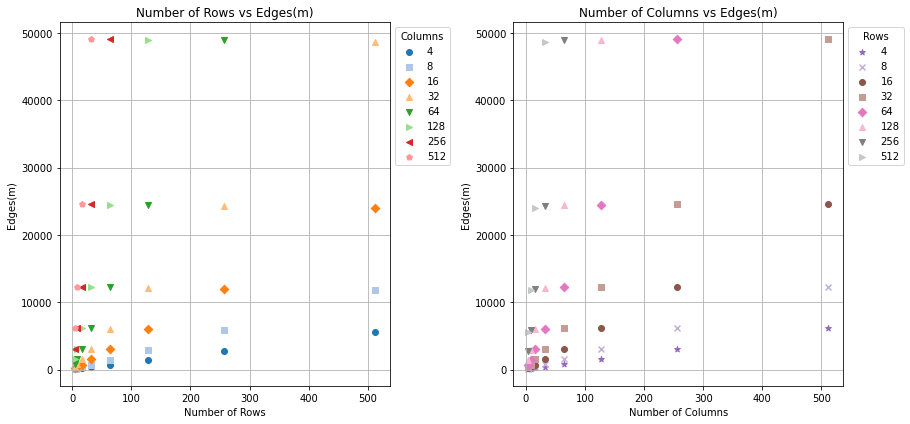
\includegraphics[width=0.8\linewidth]{edges.png}
  \label{fig:edges-example}
  \caption{Comparison of Number of edges as a function of graph parameters (rows and columns).}
\end{figure}

\subsection{Correctness}

To evaluate the effectiveness of our algorithm, we analyzed its performance based on several metrics, including the $\bar{t}$ and $\bar{s}$ ratios for BFS, as well as the $uI$ ratio, which represents the number of iterations $I$ normalized by its theoretical upper bound of $2nm$, and finally $r$ ratio.

Figure~\ref{fig:tfactor} displays the \( \bar{t} \) values. The \( \bar{t} \) ratio, being far from 1, indicates that as the number of edges increases, the proportion of edges visited during each BFS execution diverges more from its theoretical upper bound, \( m \). On the other hand, \( \bar{s} \), which measures the proportion of visited vertices, tends to be closer to 1 as the problem size increases. 

When analyzing the impact of graph dimensions on these metrics, the \emph{Number of Rows vs s} graph in Figure~\ref{fig:sfactor} demonstrates that increasing the number of rows does not significantly affect $\bar{s}$; in fact, $\bar{s}$ appears to decrease. Conversely, increasing the number of columns leads to an increase in $\bar{s}$, likely because additional columns require BFS to take more steps, thereby covering more nodes before reaching the sink. This does not occur when only the number of rows is increased since this does not necessarily increase the path length to the sink.

\begin{figure}[H]
  \centering
  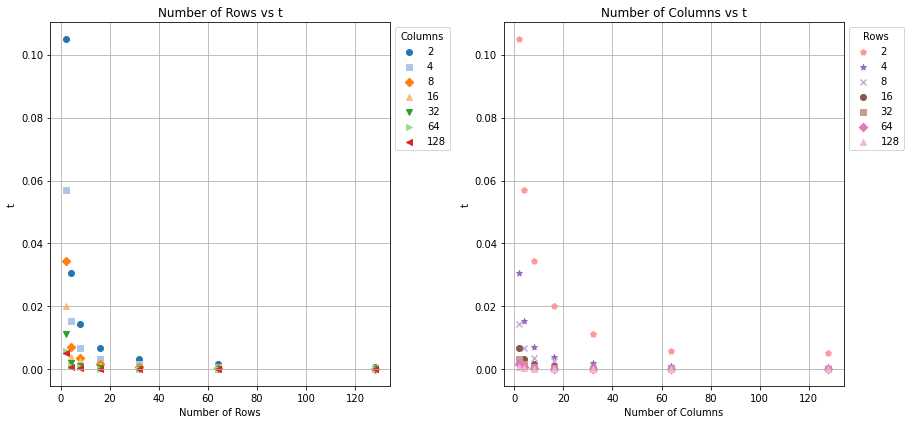
\includegraphics[width=1.0\linewidth]{t.png}
  \caption{Comparison of $t$-factor as a function of graph parameters (rows and columns).}
  \label{fig:tfactor}
\end{figure}

\begin{figure}[H]
  \centering
  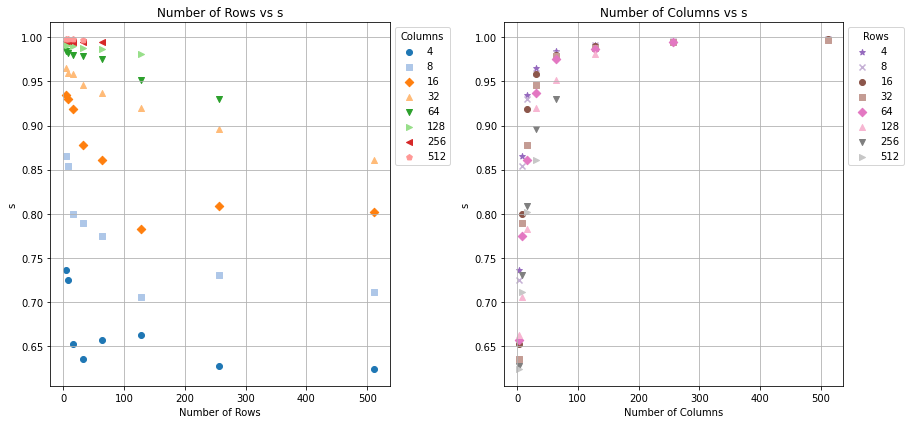
\includegraphics[width=1.0\linewidth]{sfactor.png}
  \caption{Comparison of $s$-factor as a function of graph parameters (rows and columns).}
  \label{fig:sfactor}
\end{figure}

Figure~\ref{fig:uIfactor} displays the \( uI \) ratio. This indicates the correctness of the number of augmentations for the Edmonds-Karp algorithm. \(uI\) computes the number of augmentations considering a single critical edge at a time, in case there are more multiple critical edges, the actual number of augmentations gets lower. We can see that our algorithm maintains below the \(uI\) limit, but also not very often get more than one critical edge.

\begin{figure}[H]
\centering
  \centering
  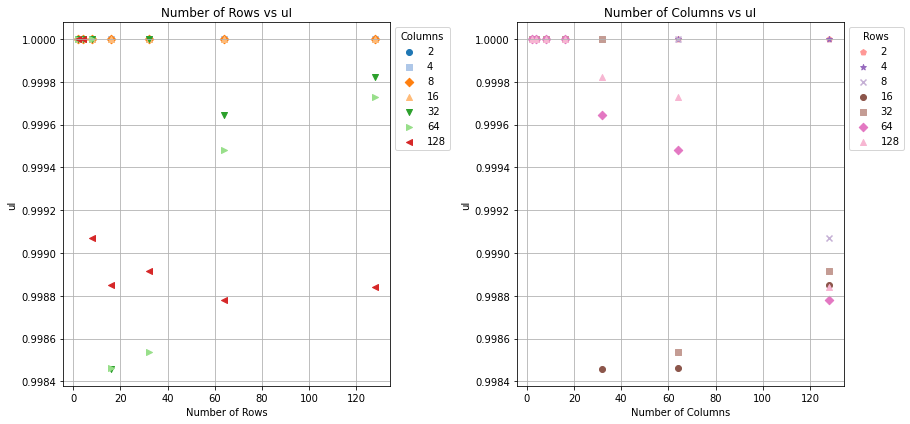
\includegraphics[width=1.0\linewidth]{uIfactor.png}
  \caption{$uI$-factor as a function of graph parameters (rows and columns).}
  \label{fig:uIfactor}
\end{figure}

A more interesting result is in Figure~\ref{fig:edges_uI} where we change the capacities and compare the graph size with \(uI\). Here we can see that using a maximum capacity of 100 and 1000 gets the lower \(uI\) values; as the maximum capacity of edges increases, meaning higher variability on values, the lower the chances of repeating edges. 

\begin{figure}[H]
\centering
  \centering
  \includegraphics[width=0.5\linewidth]{edges_uI.png}
  \caption{$uI$-factor as a function of the number of edges with different maximum capacities.}
  \label{fig:edges_uI}
\end{figure}

Figure~\ref{fig:r_factor} depicts the \( \bar{r} \) factor, which is a measure of the criticality fraction of the graph. The values, being negligible, indicate that most edges with \( C > 0 \) do not repeatedly become critical edges, maintaining low $r_a$ ratios.

\begin{figure}[H]
\centering
  \centering
  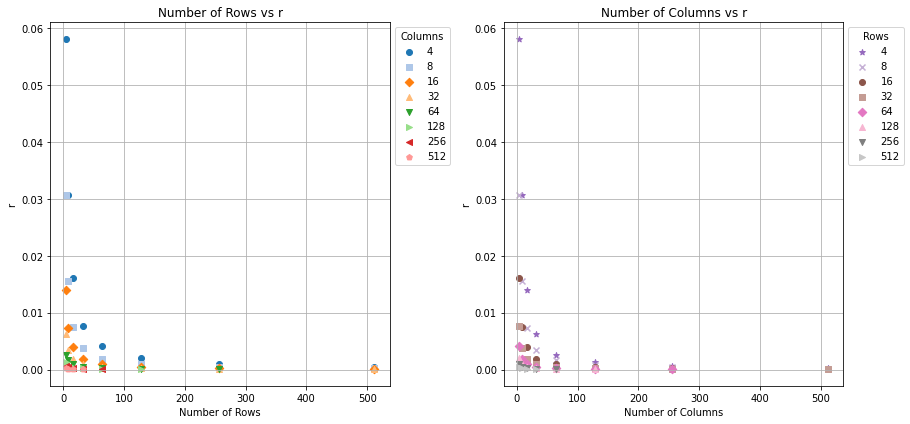
\includegraphics[width=1.0\linewidth]{rfactor.png}
  \caption{$r$-factor as a function of graph parameters (rows and columns).}
  \label{fig:r_factor}
\end{figure}

\subsection{Time Complexity}

Figure~\ref{fig:pessimistic} presents a comparison between the pessimistic time complexity and the graph size (number of edges), categorized by edges' maximum capacity. This comparison shows the discrepancies between theoretical predictions and practical outcomes, whereas the more edges are added, the less accurate the upper bound used in the pessimistic time complexity gets:

\begin{figure}[H]
\centering
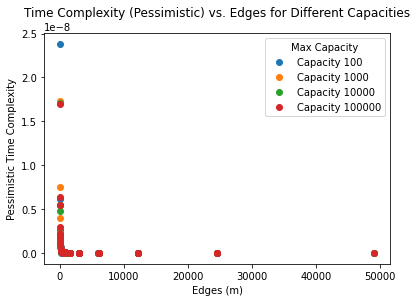
\includegraphics[width=0.6\linewidth]{pessimistic_time.png}
\caption{Time Complexity (Pessimistic) as a function of the number of edges with different maximum capacities.}
\label{fig:pessimistic}
\end{figure}

Figure~\ref{fig:opcount_time} presents the time complexity related to operation counts. Each maximum capacity level tends to stabilize at a constant value, although some data points (green) may be covered by others (red and orange). We have omitted similar analyses for the time complexity regarding residual operations, as their results are very similar. Most experiments made in Mesh graph did not get multiple critical edges in each iteration, meaning $\dfrac{\bar{r}}{2}nm$ is close to \(I\), except for the case of maximum capacity 100 (as shown in Figure~\ref{fig:edges_uI}).

\begin{figure}[H]
\centering
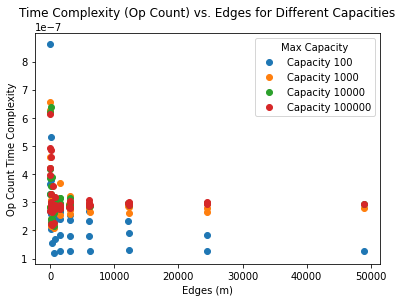
\includegraphics[width=0.6\linewidth]{opcount_time.png}
\caption{Comparison of Time Complexity (Counting Operations) as a function of the number of edges with different maximum capacities.}
\label{fig:opcount_time}
\end{figure}

The final plot regarding execution time, Figure~\ref{fig:elapsed_time}, depicts the real elapsed time, with the number of edges as the x-axis. An increase in maximum capacity generally leads to an increase in elapsed time up to a certain threshold, 10000 seems to be a reasonable value. Subsequent analysis will explore how increases in maximum capacity correlate with the number of BFS operations and augmentations.

\begin{figure}[H]
\centering
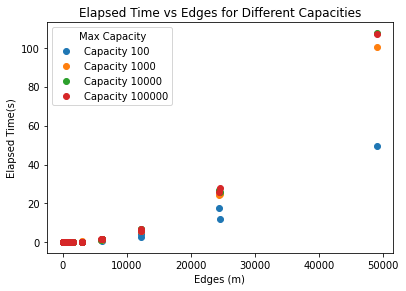
\includegraphics[width=0.6\linewidth]{elapsed_time.png}
\caption{Comparison of Elapsed Time as a function of the number of edges with different maximum capacities.}
\label{fig:elapsed_time}
\end{figure}

\subsection{Max Flow Algorithm}

Figure~\ref{fig:Cfactor} illustrates the variation of the \(C\) factor as parameters change. As the number of rows increases, the \(C\) factor stabilizes within a specific range of around 0.45 to 0.55, showing only minor variations thereafter. There is no indication of which parameter is more relevant to the \(C\) factor besides using small values (2 or 4):

\begin{figure}[H]
\centering
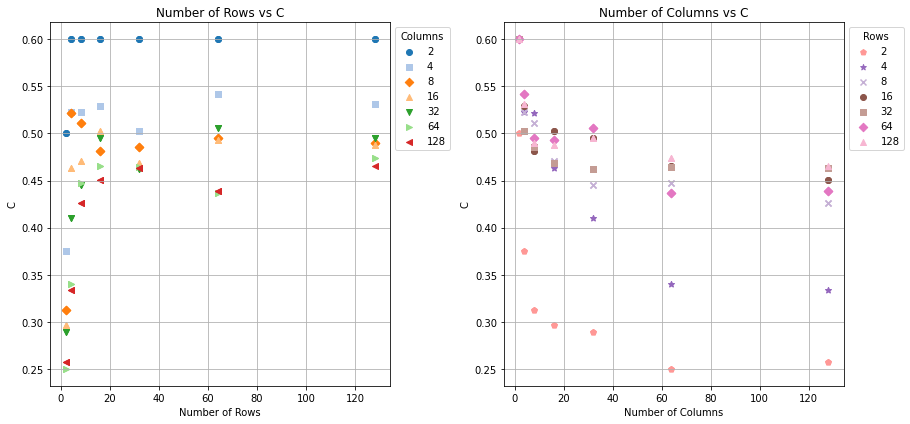
\includegraphics[width=1.0\linewidth]{Cfactor.png}
\caption{\(C\)-factor as a function of graph parameters (rows and columns).}
\label{fig:Cfactor}
\end{figure}

We also investigated whether variations in the flow capacities of the edges could influence the \(C\) factor (Figure~\ref{fig:edgesCfactor}). While our experiments generally provided no clear evidence that changes in flow capacities significantly impact the \(C\) factor, it is possible to see that the graphs using the lowest capacity of 100, represented by blue dots, tend to exhibit slightly higher \(C\) values after increasing the number of edges \(m\). This aligns with lower values obtained in \(uI\) ratio (Figure~\ref{fig:edges_uI}). Lower values for maximum capacity might lead to less variability in edge capacities, increasing the chances of getting repeated bottlenecks (repeated values). Those results are applied to our experiments in Mesh graphs, maybe by computing \(C\) in a more diverse number of graphs and capacity distributions, different \(C\) patterns might emerge.

\begin{figure}[H]
\centering
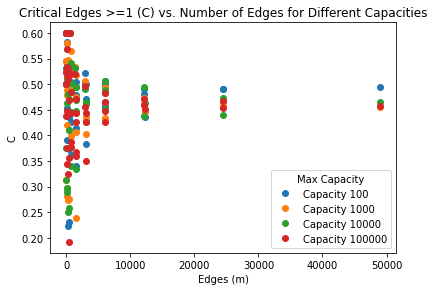
\includegraphics[width=0.6\linewidth]{edges_C.png}
\caption{Comparison of \(C\)-factor as a function of the number of edges.}
\label{fig:edgesCfactor}
\end{figure}


\section{Supplementary Analysis}

Figure~\ref{fig:maxflow} illustrates the max flow results from each experiment. Here, increasing the number of rows leads to a max flow increase. This makes sense because as more rows are added, the higher the number of incoming edges into the sink node. On the other hand, increasing the number of columns won't increase the number of sink's edges, and only should increase the chances of obtaining a lower \emph{minimum graph's cut}, as more edges are added to the graph. This could explain the behavior of \emph{Number of Columns vs Max Flow} graph, where the increasing number of columns does not increase the maximum flow.
\begin{figure}[H]
\centering
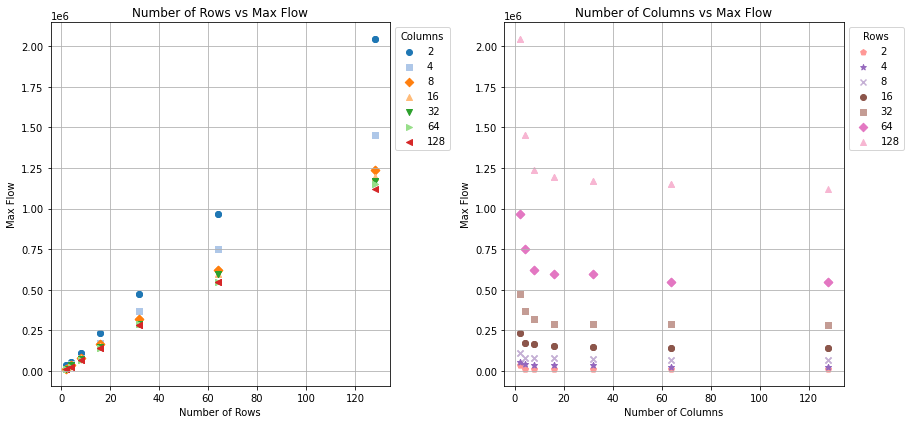
\includegraphics[width=1.0\linewidth]{maxflow.png}
\caption{Comparison of Max Flow as a function of graph parameter (rows and columns).}
\label{fig:maxflow}
\end{figure}

Another important aspect that changes the maximum flow should be the maximum capacity of the edges as shown in Figure~\ref{fig:emaxflow}:

\begin{figure}[H]
\centering
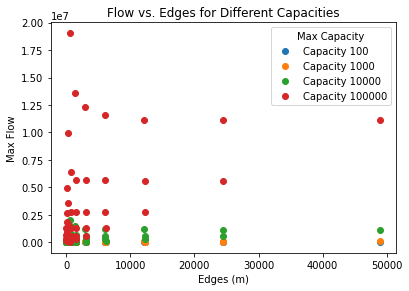
\includegraphics[width=0.6\linewidth]{edges_maxflow.png}
\caption{Comparison of Max Flow as a function of number of edges.}
\label{fig:emaxflow}
\end{figure}

Interestingly, while we expected a similar relationship in the number of augmentations, the results were inconclusive. From Figure~\ref{fig:augmentations}, it is not clear which parameter contributes more significantly to the number of augmentations, as both rows and columns appear to have a considerable impact.

\begin{figure}[H]
\centering
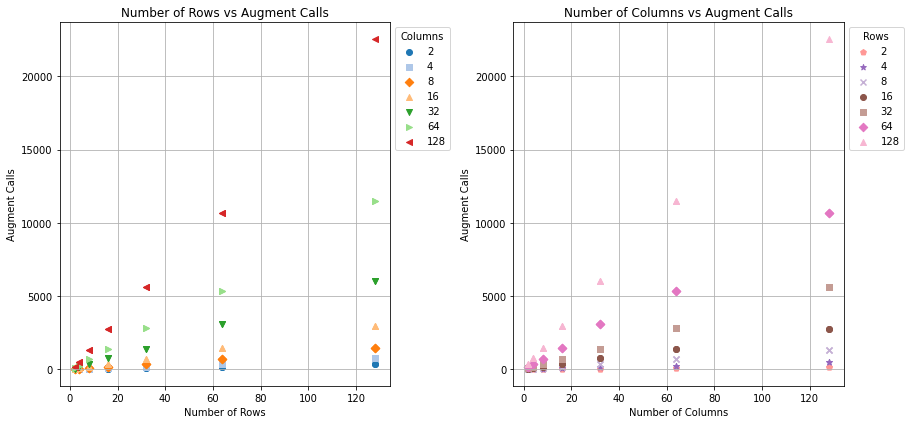
\includegraphics[width=1.0\linewidth]{augmentations.png}
\caption{Comparison of Augmentations as a function of number of edges.}
\label{fig:augmentations}
\end{figure}

Figure~\ref{fig:eaugmentations} further highlights that increasing the capacity leads to an increase in the number of augmentations. However, this increase is not a strict relation; the augmentation from 100 to 1.000 is significantly greater than from 1.000 to 10.000, and almost nonexistent from 10.000 to 100.000, suggesting diminishing returns as capacity increases.

\begin{figure}[H]
\centering
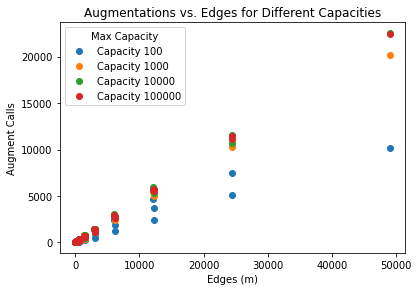
\includegraphics[width=0.6\linewidth]{edges_aug.png}
\caption{Augmentation results as Flow capacities increase.}
\label{fig:eaugmentations}
\end{figure}

Figure~\ref{fig:bfs_operations} shows the number of BFS operations over our tests, suggesting that both rows and columns lead to more operations for Edmonds-Karp, which makes sense because both contribute to increasing the graph's size, so there will be more BFS iterations. A similar behavior is observed in a previous analysis, increasing the maximum capacity leads to an increase in the number of BFS operations, achieving its peak close to 10.000.

\begin{figure}[H]
\centering
  \centering
  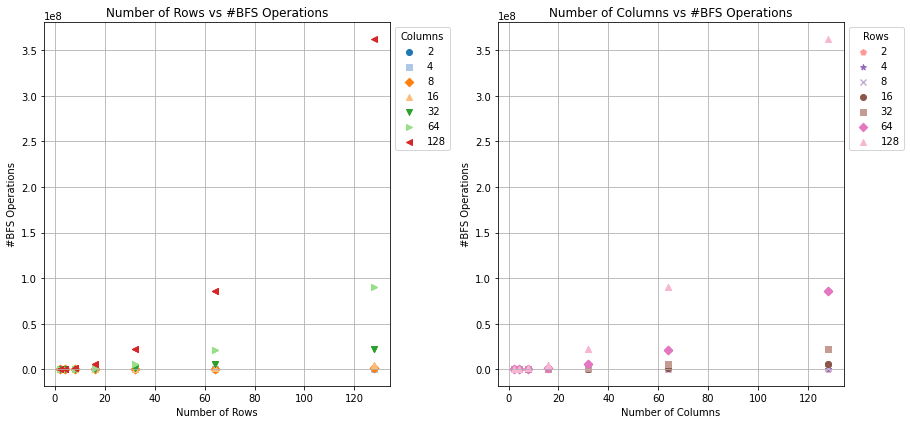
\includegraphics[width=1.0\linewidth]{bfs_operations.png}
  \label{fig:bfs_operations}
  \caption{Comparison of BFS Operations as a function of graph parameters (rows and columns).}
\end{figure}

\section{Observations and Conclusion}

Throughout the experiments, one significant realization was an error in the initial implementation of BFS, where nodes were considered only after being removed from the open list. This led to unexpectedly high numbers of iterations, affecting the experiment's practicality under higher parameter settings.  The mistake was found after computing \(t\) and \(s\) factors (found two days before the deadline).

Moreover, setting up the experiments was challenging, particularly in isolating variables and deciding on the appropriate tests to run. It was difficult to establish relationships between inputs and outcomes. Still, we only conducted very strict experiments in one type of graph and did not repeat tests under each graph setting, which could be useful. 

From the data collected, it was evident that the theoretical bounds of algorithm performance often deviate significantly from practical outcomes (Figure~\ref{fig:pessimistic}). The results in Figure~\ref{fig:maxflow} indicate that adding rows leads to increased max flow, but not necessarily the same with adding columns. The experiment also revealed that adjustments in the maximum capacities of the edges led to higher maximum flows and increased the number of augmentations up to a certain limit (Figures~\ref{fig:emaxflow} and \ref{fig:eaugmentations}).

\end{document}